\subsection{What Lite Has Learned}\label{sec:explain}

% Generated by paper_mdpi/tools/make_tables.py. Do not edit by hand.
\begin{table}[H]
\caption{The strongest distinct character n-gram features of each class in Lite\label{tab:ngrams}}
\small
\begin{tabularx}{\textwidth}{clccL}
\toprule
Rank & n-gram & $w_{k,g}$ & Merged & Interpretation \\
\midrule
\multicolumn{5}{l}{\emph{ham}} \\
1 & \texttt{..} & 0.81 & 4 & ellipsis in informal writing (ok..., lor...) \\
2 & \texttt{i\textvisiblespace{}} & 0.68 & 3 & pronoun I \\
3 & \texttt{:)} & 0.45 & 1 & emoticon \\
4 & \texttt{my\textvisiblespace{}} & 0.39 & 4 & pronoun my \\
5 & \texttt{so} & 0.38 & 3 & so, sorry, some \\
6 & \texttt{\textvisiblespace{}m} & 0.38 & 1 & start of my, me, much, make \\
7 & \texttt{me\textvisiblespace{}} & 0.36 & 3 & me, and come, time, home \\
8 & \texttt{\textvisiblespace{}it} & 0.32 & 1 & pronoun it \\
\midrule
\multicolumn{5}{l}{\emph{smishing}} \\
1 & \texttt{\textvisiblespace{}0} & 1.24 & 2 & start of a phone number (0800..., 087...) \\
2 & \texttt{00} & 1.03 & 3 & amounts and numbers (\pounds1000, 0800) \\
3 & \texttt{08} & 0.84 & 3 & phone numbers 08... \\
4 & \texttt{09} & 0.83 & 2 & phone numbers 09... \\
5 & \texttt{20} & 0.75 & 1 & amounts and years (\pounds2000, 2003) \\
6 & \texttt{all\textvisiblespace{}0} & 0.74 & 3 & request to call a number (call 0...) \\
7 & \texttt{claim} & 0.65 & 9 & prize claim \\
8 & \texttt{50} & 0.60 & 1 & amounts and rates (\pounds500, 150ppm) \\
\midrule
\multicolumn{5}{l}{\emph{spam}} \\
1 & \texttt{txt} & 1.10 & 7 & txt: subscription and chat services \\
2 & \texttt{\textvisiblespace{}8} & 1.10 & 2 & start of a short code (8007, 86688) \\
3 & \texttt{\textvisiblespace{}to\textvisiblespace{}8} & 0.90 & 4 & reply to a short code (to 86688) \\
4 & \texttt{tone} & 0.89 & 12 & ringtone \\
5 & \texttt{88} & 0.82 & 1 & digits of a short code (86688) \\
6 & \texttt{50} & 0.77 & 1 & prices (150p, \pounds1.50) \\
7 & \texttt{10} & 0.73 & 1 & prices (\pounds100, \pounds10) \\
8 & \texttt{ms} & 0.71 & 1 & sms, msg \\
\bottomrule
\end{tabularx}
\noindent{\footnotesize{Coefficients of the one-versus-rest linear SVM of Lite (seed 1) on lower-cased character n-grams, read from the saved weights after the evaluation (post hoc, no training). Overlapping n-grams of a class (one inside the other or overlapping within a word, such as claim, laim, aim and clai) are merged: among the 60 strongest n-grams of the class, each joins the strongest group it overlaps; a group is shown by its longest n-gram within 75\% of the group's largest weight, with that weight. Merged: number of n-grams in the group. Interpretation: from the words of the training messages of the class that contain the n-gram most often. \textvisiblespace{} marks a space. Unmerged list: Table~\ref{tab:ngrams-full}.}}
\end{table}


Table~\ref{tab:ngrams} lists, for each class, the \val{ngm-top} strongest distinct features of the Lite model of seed 1, read from its saved weights after the evaluation (Section~\ref{sec:explain-method}; post hoc, no training). Overlapping n-grams of a class, such as claim, laim and aim, are merged into one feature; the unmerged list is in Table~\ref{tab:ngrams-full}. The vocabulary has \val{ex-n-features} character n-grams. For ham, the features are marks of personal conversation: ellipses (\val{ngm-ham-1}), emoticons (\val{ngm-ham-3}) and the pronouns \emph{I}, \emph{my}, \emph{me} and \emph{it}. For smishing, \val{ngm-smishing-digits} of the \val{ngm-top} features are digit sequences of phone numbers and amounts, such as the start of a number (\val{ngm-smishing-1}) and the prefixes \val{ngm-smishing-3} and \val{ngm-smishing-4}; the others are the request to call a number (\val{ngm-smishing-6}) and the word \emph{claim}. For spam, they come from subscription and ringtone services: \emph{txt}, replies to short codes (\val{ngm-spam-3}), \emph{tone} and prices. Lite has thus learned cues of what a message asks the recipient to do (call a number, claim a prize, reply to a short code) more than particular topics. Some of these cues, such as the digit patterns of phone numbers, are specific to the senders and numbering plans of the corpus and cannot be expected to carry over to other countries (Section~\ref{sec:kz}).

\begin{figure}[H]
\centering
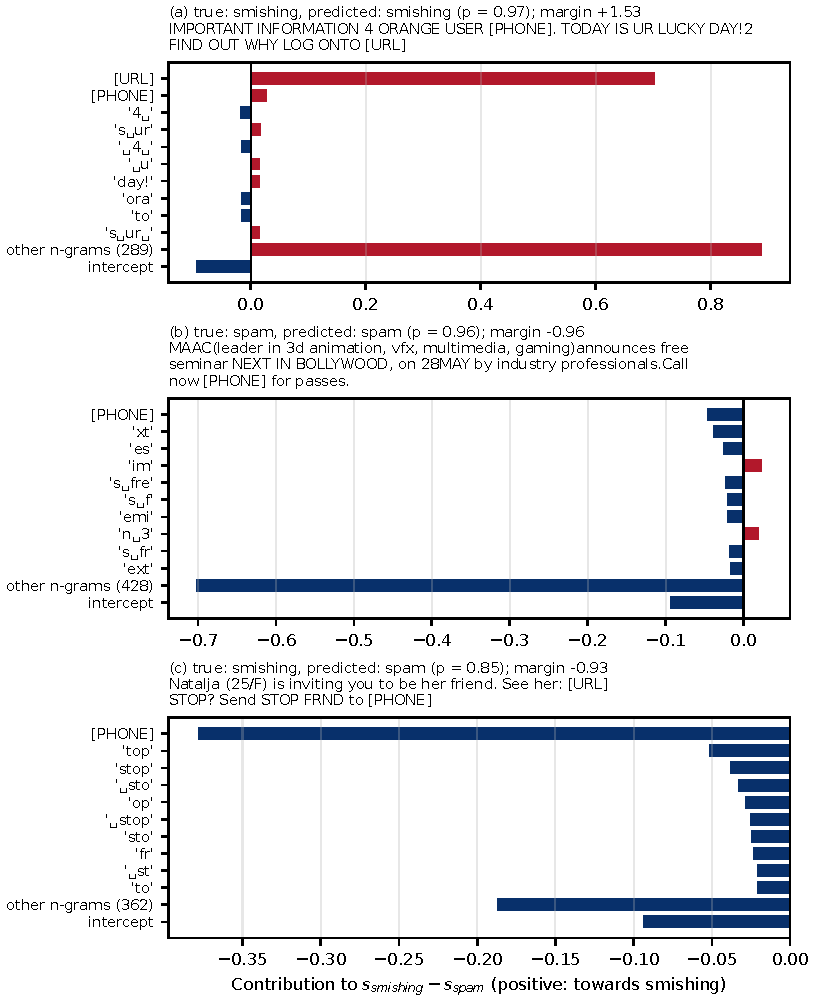
\includegraphics{figures/explanation_examples}
\caption{Contributions of the words of three test messages of the Mendeley corpus \cite{mendeley2022} to the decision of Lite between smishing and spam, chosen by a fixed rule (median confidence in each group): (\textbf{a}) a smishing message classified correctly, (\textbf{b}) a spam message classified correctly, (\textbf{c}) a smishing message classified as spam. The contribution of a word is the sum of the contributions (\ref{eq:contrib}) of the character n-grams that overlap it; an n-gram that spans two words is split equally between them. The bars show the \val{ex-top-words} words with the largest absolute contributions; the other words contribute \val{ex-sm-rest}, \val{ex-sp-rest} and \val{ex-err-rest} in (\textbf{a}), (\textbf{b}) and (\textbf{c}), and the intercept $b_{\mathrm{smishing}}-b_{\mathrm{spam}}$ is \val{ex-icpt}, so that the margins $s_{\mathrm{smishing}}-s_{\mathrm{spam}}$ are \val{ex-sm-margin}, \val{ex-sp-margin} and \val{ex-err-margin}. Messages are quoted verbatim from the corpus, including the original spelling; phone numbers, links and names are masked.\label{fig:explain}}
\end{figure}

Figure~\ref{fig:explain} decomposes three decisions by words. In the correctly classified smishing message (a), one of \val{ex-sm-n} in its group, with confidence \val{ex-sm-conf}, the masked link gives the largest contribution towards smishing (\val{ex-sm-url}); no other word contributes more than \val{ex-sm-second}, and the rest of the evidence is spread over the other words of the message. In the correctly classified spam message (b), with confidence \val{ex-sp-conf}, the eight largest contributions all point towards spam and none exceeds \val{ex-sp-max}: the decision is the sum of many small contributions of advertising wording. The misclassified smishing message (c) is one of \val{ex-err-n} smishing messages labelled spam by Lite on seed 1. The word \emph{STOP}, which occurs twice, pushes it towards spam by \val{ex-err-stop} and the short number at the end by \val{ex-err-phone}, as in the opt-out instructions of subscription services. The message, an invitation from a contact service with a link, lies on the boundary between the two malicious classes discussed in Section~\ref{sec:duplicates}. Because the evidence of a message is spread over many overlapping n-grams, editing a few characters changes only a small part of its score, which is consistent with the robustness of Lite in Sections~\ref{sec:published} and \ref{sec:robustness}.
